\chapter{State of the Art}

% AMAIA: For the state of the art, I think that you should re-organize it to cover the main different challenges of video analysis, and explain what people do to tackle each (even though you end up citing the same paper more than once in the process). You should also explain what you do in your project, and how it resembles or differs from what others did.

% 1. How do people use information in different frames? Some use 2D convolutions and merge them somehow, others use 3D conv. Here you can talk about pretrained networks (some people use VGG imagenet, there's people who have trained other models for Sports1M, right?)
% 2. How is motion encoded ? Some works directly use optical flow, while others directly input the visual data.
% 3. How do people ensure temporal consistency? LSTMs or GRUs
% 4. Particularly for activity detection, how do people do this? I remember the paper from columbia, where there are several stages. Maybe a strength of your work is that you train a single network that does it all (you just postprocess the output).
% ...


Many works in the literature have explored activity and action recognition problems using deep learning strategies. Most of them used an approach of two stages (encoder and decoder) trained on a dataset of videos. The first stage, the one being consider a decoder, is the stage that tries to encode the visual and temporal information from the input videos into some features vectors or information. The second stage, also known as decoder, casts a prediction of the output, which can be a classification of the video or a temporal localization of an activity.

\section{Convolutional Neural Networks applied to Videos}

A popular solution as encoder are Convolutional Neural Networks (or also known as CNNs) as it has been widely demonstrated that applying CNN networks to images and videos produces good results in classifications tasks. A very well known and used CNN network is the VGG\cite{Simonyan14c} network which was top scored on ImageNet Challenge in 2014 on classification task. This network uses 2D convolutional kernels to extract spatial correlations from images.

To understand better how Convolutional Neural Networks works, the Figure~\ref{fig:cnn_architecture} represent its common architecture. Starting from a 2D input matrix such as an image, the CNN is made up by layers, which each one presents a different number of filter or also called kernels.
During the forward pass, it is convolved each filter accross the width and height of the input volume and compute do products between the entries of the filters and the input at any position. As it is slided the filter over the width and height of the input volume, it will be produced a 2-dimensional activation map that gives the responses of the filter at every spatial position.
Intuitively, the network will learn filters that activate when they see some type of visual feature. It is also common insert pooling layers in-between successive convolutional layers.
Its function is to progressively reduce the amount of parameters and computation of the network using subsampling operations. This subsampling operations take the parameters on a kernel size and perform an operation such as computing the maximum or the mean to reduce the kernel size into a single feature. With this operation a subsampling is performed.

There exist some works which use 2D Convolutional Neural Networks over the frames~\cite{gkioxari2015contextual}~\cite{yeung2015end}~\cite{ballas2015delving} to extract spatial correlations from video data. As the video also presents temporal correlation, different approaches have been tried to exploit it. The first approach is weighting the frames at the input\cite{yeung2015every} so information of a chunk of frames is given to the neural network.

\begin{figure}[ht]
\begin{center}
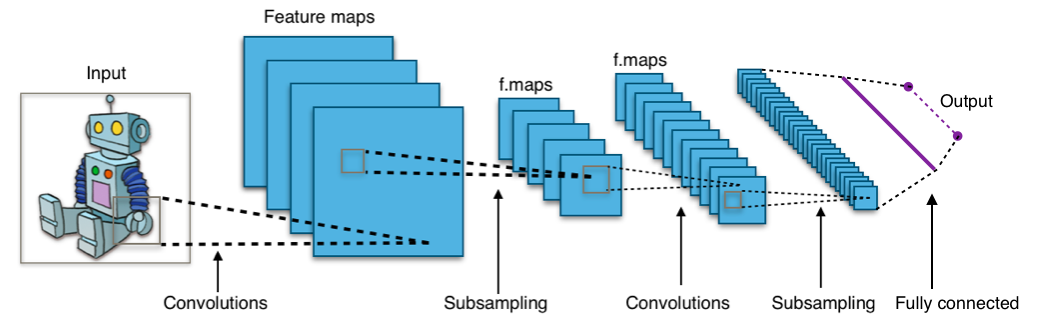
\includegraphics[width=1\linewidth]{img/stateofart/cnn_architecture}
\end{center}
\caption{Example of the Architecture of a Convolutional Neural Network}
\label{fig:cnn_architecture}
\end{figure}

Another approach is computing the optical flow to codify temporal correlations and train convolutional neural networks\cite{simonyan2014two}\cite{Ng_2015_CVPR} with even two streams\cite{wang2015towards}, one for the frame and the other for the optical flow. These techniques exploit temporal information but they are limited to the information in a 2D projection, without letting the neural network learning about temporal information.

On the other hand, a recently proposed a CNN tries to exploit both spatial and temporal correlations using exclusively a Convolutional Network. This is the 3D convolutional network, also referenced as C3D\cite{tran2014learning}. This network uses 3D kernels rather than 2D to extract videos information and try to learn from both the spatial and temporal dimensions. It has been widely used\cite{baccouche2011sequential}\cite{tran2015deep}\cite{tran2014learning}\cite{shoutemporal} for applications such as video classification. On some other research papers\cite{yao2015describing}\cite{zhang2016modelling} both approaches have been tried using 2D and 3D convolutional networks.

For this C3D network, the input data are clips of videos where all the frames are provided without any previous codification and even it has been proposed a combination of 2D and 3D Convolutional Neural Networks\cite{Ng_2015_CVPR}\cite{yao2015describing}. Also it has been tried to extract motion 3D features from videos to feed as input of the 3D CNN\cite{yao2015describing}.

In addition to spatial and temporal correlations, it has been seen that some approaches extract information from the audio track to explode the information it may give. This technique of combining both video and audio is becoming trendy on the latest activity detection on video datasets\cite{xu2015uts}. The idea of extracting information from the audio in addition to the video seems really interesting but its success on the results are very related to the coherence between the audio and video tracks.

The recent work presented in \cite{shoutemporal} is based on Convolutional Neural Networks, more concretely on the C3D network previously explained. It proposes to divide each video in multiple sequences of different lengths and predict for each one whether if they depict an activity or not. In affirmative class, another classification stage determines which of the activities is represented in the video segment. As the first stage, they propose to subsample the segments obtained from the video to put it as input for the C3D. The next stage consist on three parallel networks which are trained separately. All the three networks are trained doing a fine tunning from the original C3D network\cite{tran2014learning}.

\begin{figure}[hb]
\begin{center}
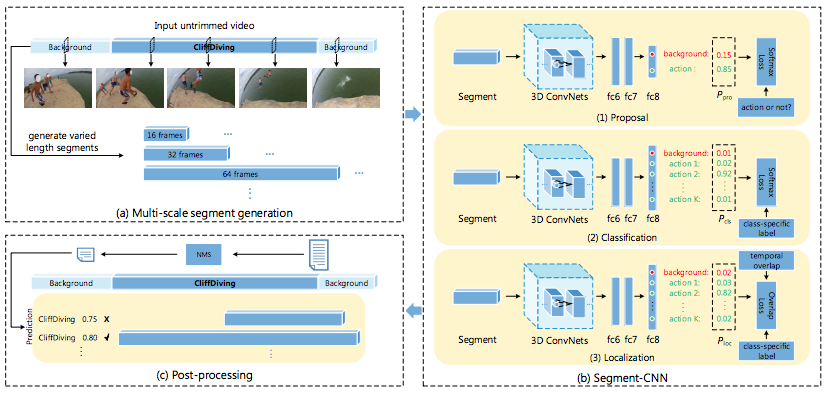
\includegraphics[width=1\linewidth]{img/stateofart/multistage}
\end{center}
\caption{Multi-stage architecture to temporal action location using CNNs}
\label{fig:multistage}
\end{figure}


\section{Recurrent Neural Networks applied to Videos}

A more complex and different approach to address activity classification and temporal localization on videos is using RNNs. This networks are characterized by being trained with sequences of related data and having memory cells. RNNs are mainly used to learn from temporal sequences as text generation or speech recognition, but they have also been used in tasks related to video.

The most efficient implementation of Recurrent Neural Network found at the literature is the Long Short Term Memory cells\cite{hochreiter1997long}, or also known as LSTM. This cell, represented in the Figure~\ref{fig:lstm_chain}, has as input the combination of the previous cell output and the layer's input in addition to a cell state which is propagated at every temporal step and represents the memory of the cell.
When forwarding information, the first step is to decide what information is going to be thrown away from the cell state. This decision is made by a sigmoid layer called the \textit{forget gate layer}.
The next step is to decide what new information is going to be stored in the cell. First a sigmoid layer called \textit{input gate layer} decides which values are going to be updated. Next, a $\tanh$ layer creates a vector of new candidate values that could be added to the state. As the next step, both will be combined to create an update to the cell state.
Finally, the output will be computed based on the cell state, but will be a filtered version. First a sigmoid layer decides what parts of the cell state are going to the output and multiply it by the cell state after a $\tanh$ layer.
This cells also presents propagation of information along temporal sequences and can be represented forming chain as can also seen on Figure~\ref{fig:lstm_chain}, where each element represents a single time step.

%It also has a memory state which is propagated at every temporal step after performed first some operation. The first step is to compute the forget gate which decides if the information of the memory

%This cells present internal gates that control the propagation of information along the network and also along the temporal sequence forming a chain as is shown in Figure~\ref{fig:lstm_chain}.

\begin{figure}[ht]
\begin{center}
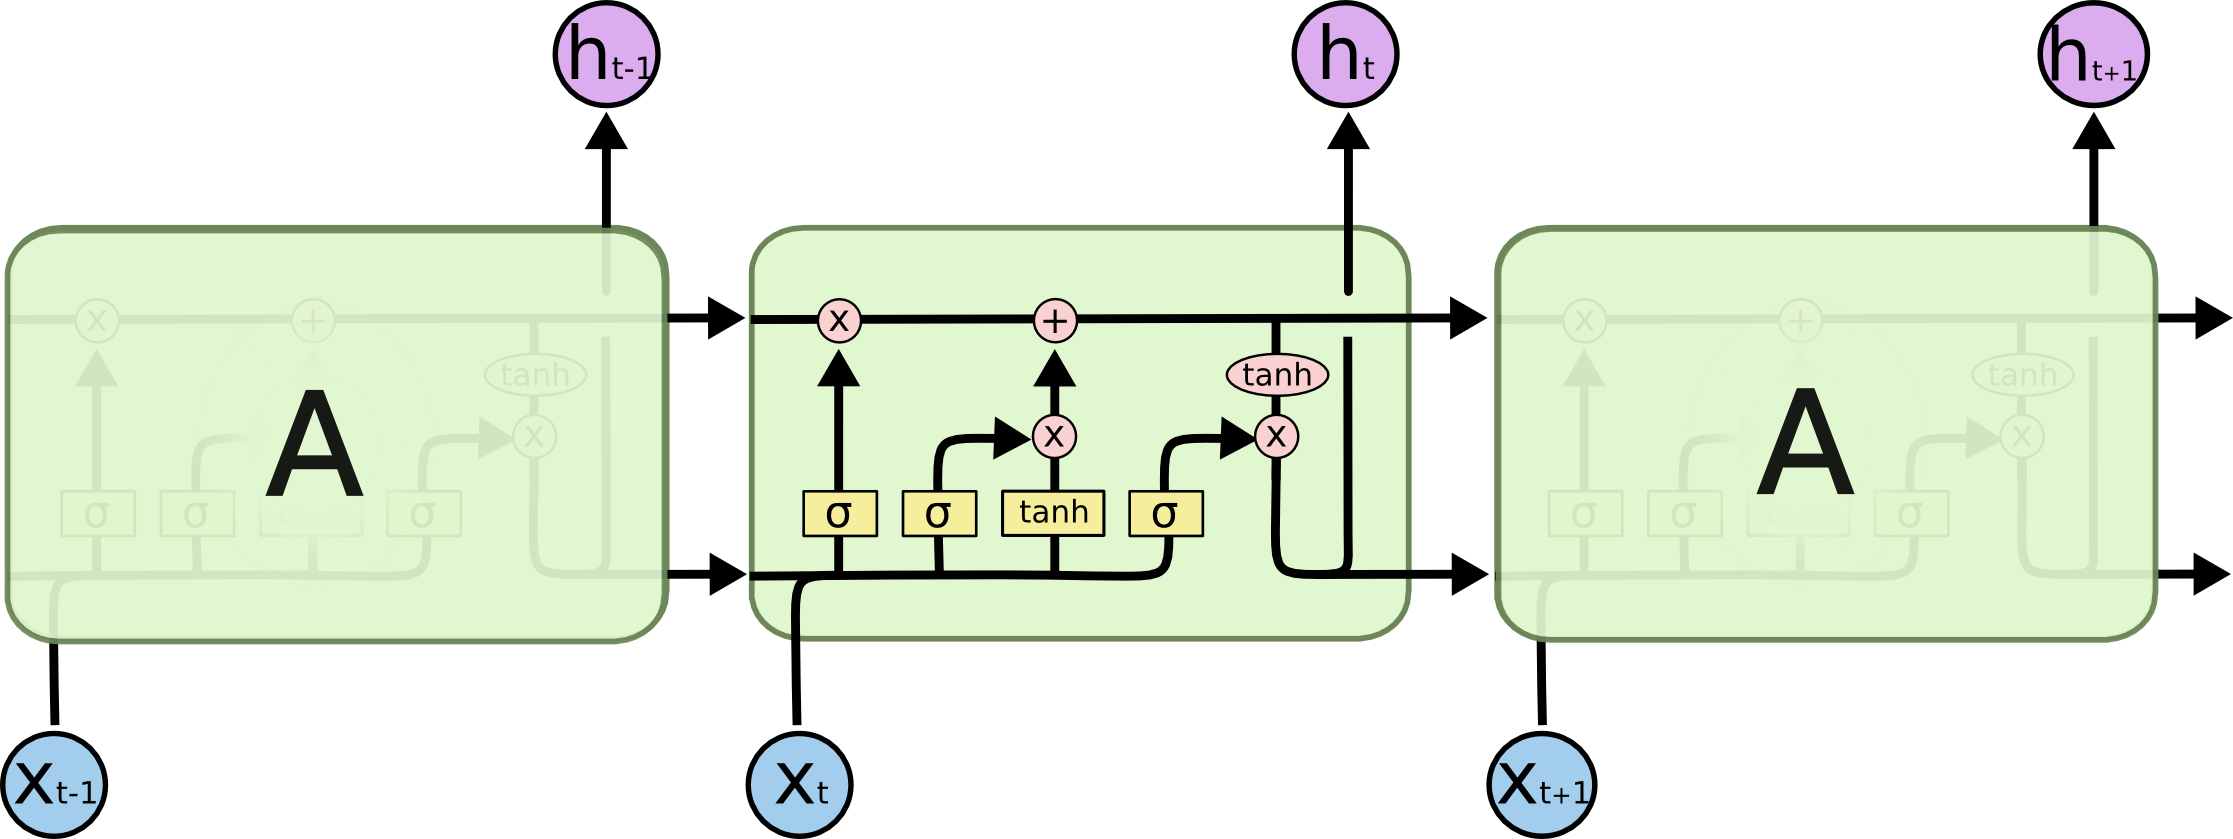
\includegraphics[width=0.8\linewidth]{img/stateofart/lstm_chain}
\end{center}
\caption{Example of the Architecture of a Convolutional Neural Network}
\label{fig:lstm_chain}
\end{figure}

Most of the literature that uses RNN on video, make their implementation using LSTM cells, but with different approaches. Some works propose to predict activities using LSTMs after features by CNNs\cite{yao2015describing}, while others propose to add an attention model before the recurrent stage to let the network learn where to focus the attention\cite{sharma2015action}\cite{piergiovanni2016temporal}. At~\cite{yeung2015every} for example, a Recurrent Neural Network using LSTMs is used after a 2D CNN to predict the activity on videos returning, from the temporal sequence of input frames, a sequence of activities done at each input frame.
Another approach found in the literature is using LSTMs and reinforcement learning to temporally localize activities on videos\cite{yeung2015end} achieving state of the art performance. This achieves very good results without the requirement to have a prediction after seeing all the video frames because with little iterations, the network predicts where the activity is temporally located.

In addition to previous exposed LSTMs, there is a little variation of it which is a cell called Gated Recurrent Unit (GRU)\cite{cho2014learning}. This is a slightly variation of the LSTM which combines the forget and input gate into an update gate and has been applied in the task of video classification\cite{ballas2015delving} in conjunction with CNNs.

% AMAIA: Yes, definitely ! I think that what you will explain in later sections is primarily focused on detection, so it is relevant that you explain what people have done in the past, and how your approach differs from them. I think what is interesting in your work is that you don't train in several stages using segment candidates. You train a single network. Ok, it does not improve the results, but the approach is much nicer ideally.
